\textbf{Inizio:} 2024-04-01\\
\textbf{Fine prevista:} 2024-06-07
\subsection{Primo periodo} \label{sec:1_rtb}
\textbf{Inizio:} 2024-04-01\\
\textbf{Fine prevista:} 2024-04-19
\subsubsection{Pianificazione}
Nella fase iniziale, assume prioritaria importanza la discussione di tutte le regole precedentemente adottate e implementate nel corso del progetto, ma che non sono ancora state formalizzate mediante documentazione. Questo processo mira a produrre un documento scritto accessibile a tutti i membri del team, al fine di dissipare eventuali ambiguità riguardo l'esecuzione delle attività e l'utilizzo delle risorse.
\\
Inoltre, durante questa fase, è cruciale identificare tutti i potenziali rischi che potrebbero ostacolare il progresso del progetto, al fine di prevenirli e non essere colti impreparati. Un'altra priorità consiste nell'avviare la pianificazione delle prime attività e delle relative milestone, al fine di organizzare le risorse disponibili e fornire una stima preventiva dei tempi e dei costi. \\
Le attività previste per il primo periodo sono dunque le seguenti:
\begin{itemize}
\setlength{\itemsep}{0em}
    \item Avvio della stesura dei documenti \textit{Piano di Progetto}, \textit{Glossario}, \textit{Norme di Progetto}, \textit{Piano di Qualifica} e \textit{Analisi dei Requisiti};
    \item Realizzazione di un generatore dati in grado di simulare un sensore di temperatura;
    \item Predisposizione di un \glossterm{container} \glossterm{Docker} con all'interno un'installazione della tecnologia \glossterm{Kafka}.
\end{itemize}

\subsubsection{Rischi attesi}
I rischi che ci aspettiamo di correre in questo periodo sono i seguenti: 
\begin{itemize}
\setlength{\itemsep}{0em}
\item \textbf{RT-1}: Inesperienza;
\item \textbf{RP-1}: Stima errata delle tempistiche di progetto;
\item \textbf{RP-2}: Stima errata dei costi di progetto;
\item \textbf{RC-1}: Scarsa comunicazione interna;
\item \textbf{RC-3}: Conflitti interni.
\end{itemize}
Questo perchè, essendo all’inizio del progetto, siamo ancora incerti su molti aspetti di
quest’ultimo, ci stiamo attualmente organizzando e dobbiamo apprendere ancora molto, dunque la
probabilità di incorrere in qualche problema tra quelli riportati è abbastanza elevata.
\newpage
\subsubsection{Preventivo}
\subsubsubsection{Preventivo orario}
\begin{table}[ht!]
	\centering
	\begin{tabular}{p{4cm} p{1cm} p{1cm} p{1cm} p{1cm} p{1cm} p{1cm} p{3cm}}
		\toprule
        \textbf{Membro} & \multicolumn{6}{c}{\textbf{Ruoli}} & \textbf{Totale (persona)}\\
		& \textbf{AM} & \textbf{RE} & \textbf{PT} & \textbf{AN} & \textbf{PR} & \textbf{VE}\\
		\midrule
        Linda Barbiero          & -     & 3     & -     & 2     & -     & 1     & 6 \\
        Guglielmo Barison       & 3     & -     & 1     & 1     & 2,5   & 1     & 8,5\\
        Pietro Busato           & 3     & -     & 1     & 1     & 2,5   & 1     & 8,5 \\
        Davide Donanzan         & 3     & -     & -     & 3     & -     & 1,5   & 7,5 \\
        Oscar Konieczny         & 3     & -     & -     & 1     & -     & 1     & 5 \\
        Veronica Tecchiati      & 3     & -     & -     & 4     & -     & 1     & 8 \\
        \bottomrule
        \textbf{Totale (ruolo)} & 15     & 3     & 2     & 12   & 5     & 6,5   & 43,5 \\
	\end{tabular}
	\caption{Distribuzione delle ore del primo Sprint secondo ruolo e membro.}
	\label{table:Distribuzione delle ore del primo Sprint secondo ruolo e membro}
\end{table}
\begin{figure}[ht!]
    \centering
    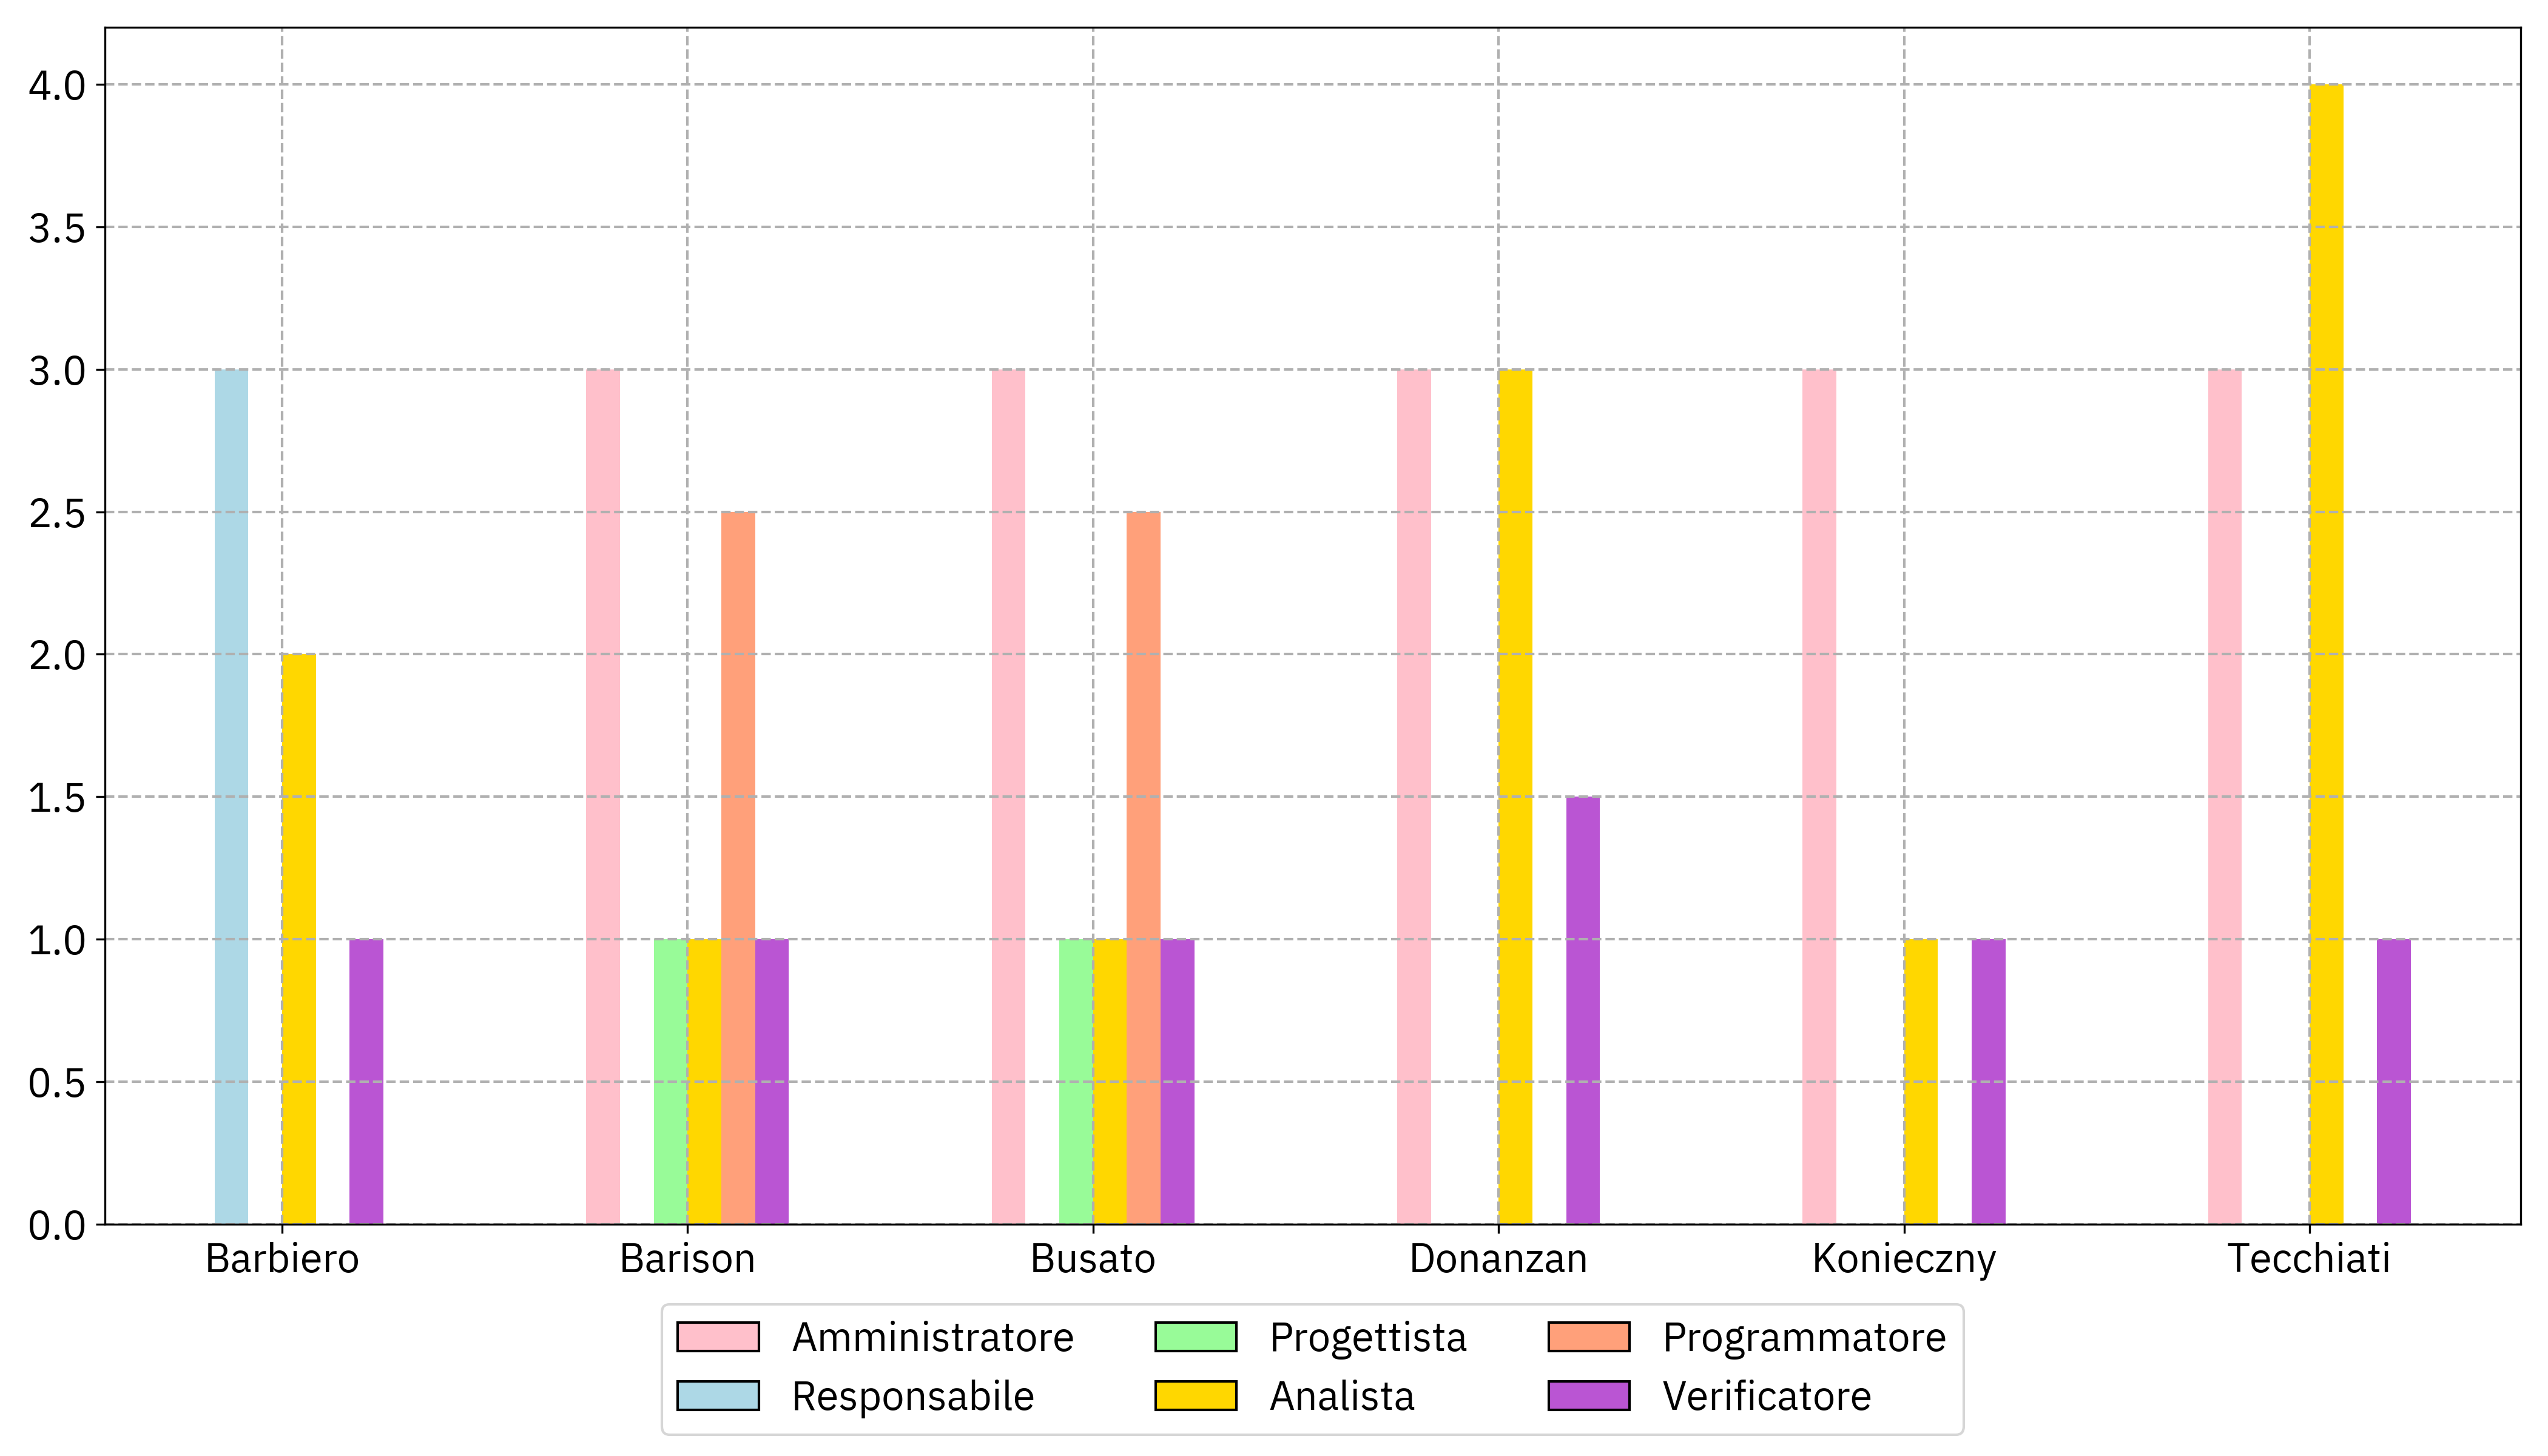
\includegraphics[width=15cm]{./asset/istogramma_periodo_1.png}
    \caption{Visualizzazione dell’impegno temporale di ciascun membro nei rispettivi ruoli assegnati
    nel primo Sprint.}
    \label{figure:Visualizzazione dell’impegno temporale di ciascun membro nei rispettivi ruoli
    assegnati nel primo Sprint}
\end{figure}
\subsubsubsection{Preventivo economico}
\begin{table}[ht!]
	\centering
	\begin{tabular}{p{4cm} p{1cm} p{2cm}}
        \toprule
        \textbf{Ruolo} & \textbf{Ore} & \textbf{Costo (€)} \\
        \midrule
        Amministratore & 15 & 450 \\
        Responsabile & 3 & 60 \\
        Progettista & 2 & 50 \\
        Analista & 12 & 300 \\
        Programmatore & 5 & 75 \\
        Verificatore & 6,5 & 97,5 \\
        \bottomrule
        \textbf{Totale} & 43,5 & 1032,5
    \end{tabular}
    \caption{Preventivo dei costi del primo Sprint secondo ruolo.}
	\label{table:Preventivo dei costi del primo Sprint secondo ruolo}
\end{table}
\subsubsection{Consuntivo}
\subsubsubsection{Consuntivo orario}
\begin{table}[ht!]
	\centering
	\begin{tabular}{p{3cm} p{1.5cm} p{1.5cm} p{1.5cm} p{1.5cm} p{1.5cm} p{1.5cm} p{1cm}}
		\toprule
        \textbf{Membro} & \multicolumn{5}{c}{\textbf{Ruoli}} & \multicolumn{2}{r}{\textbf{Totale
        (pers.)}}\\
		& \textbf{AM} & \textbf{RE} & \textbf{PT} & \textbf{AN} & \textbf{PR} & \textbf{VE}\\
		\midrule
        Linda Barbiero          & -     & 3     & -     & 2     & 0     & 0.5 \textcolor{teal}{(-0,5)}   & 5,5 \\
        Guglielmo Barison       & 3     & -     & 1     & 1     & 2,5   & 1     & 8,5\\
        Pietro Busato           & 3     & -     & 1     & 1     & 2,5   & 1     & 8,5 \\
        Davide Donanzan         & 3     & -     & -     & 3     & -     & 2 \textcolor{teal}{(-0,5)}     & 8 \\
        Oscar Konieczny         & 3,5 \textcolor{teal}{(-0,5)}  & -     & -     & 1     & -     & 1     & 5,5 \\
        Veronica Tecchiati      & 3,5 \textcolor{teal}{(-0,5)}  & -     & -     & 5 \textcolor{teal}{(-1)}    & -     & 1     & 9,5 \\
        \bottomrule
        \textbf{Totale (ruolo)} & 16    & 3     & 2     & 13   & 5     & 6,5   & 45,5 \\
	\end{tabular}
	\caption{Distribuzione delle ore del primo Sprint secondo ruolo e membro.}
	\label{table:Distribuzione delle ore consuntive del primo Sprint secondo ruolo e membro}
\end{table}
\begin{table}[ht!]
	\centering
	\begin{tabular}{p{4cm} p{1cm} p{1cm} p{1cm} p{1cm} p{1cm} p{1cm} p{3cm}}
		\toprule
        \textbf{Membro} & \multicolumn{6}{c}{\textbf{Ruoli}} & \textbf{Totale (persona)}\\
		& \textbf{AM} & \textbf{RE} & \textbf{PT} & \textbf{AN} & \textbf{PR} & \textbf{VE}\\
		\midrule
        Linda Barbiero          & 7     & 5     & 20     & 11   & 24     & 22,5   & 89,5 \\
        Guglielmo Barison       & 4     & 9     & 19     & 11   & 21,5   & 22     & 86,5\\
        Pietro Busato           & 6     & 8     & 19     & 11   & 20,5   & 22     & 86,5 \\
        Davide Donanzan         & 6     & 8     & 20     & 9    & 23     & 21     & 87 \\
        Oscar Konieczny         & 4,5   & 7     & 20     & 11   & 24     & 23     & 89,5 \\
        Veronica Tecchiati      & 4,5   & 8     & 20     & 6    & 25     & 22     & 85,5 \\
        \bottomrule
        \textbf{Totale (ruolo)} & 32    & 45    & 118    & 59   & 138     & 132,5 & 524,5 \\
	\end{tabular}
	\caption{Ore rimaste dopo il primo Sprint secondo ruolo e membro.}
	\label{table:Ore rimaste dopo il primo Sprint secondo ruolo e membro}
\end{table}
\subsubsubsection{Consuntivo economico}
\begin{table}[ht!]
	\centering
	\begin{tabular}{p{4cm} p{2cm} p{2cm}}
        \toprule
        \textbf{Ruolo} & \textbf{Ore} & \textbf{Costo (€)} \\
        \midrule
        Amministratore & 16 \textcolor{red}{(+1)} & 480 \textcolor{red}{(+30)} \\
        Responsabile & 3 & 60 \\
        Progettista & 2 & 50 \\
        Analista & 13 \textcolor{teal}{(-1)} & 325 \textcolor{teal}{(-25)} \\
        Programmatore & 5 & 75 \\
        Verificatore & 6,5 & 97,5 \\
        \bottomrule
        \textbf{Totale} & 45,5 & 1087,5
    \end{tabular}
    \caption{Preventivo a finire dei costi del primo Sprint secondo ruolo.}
	\label{table:Preventivo a finire dei costi del primo Sprint secondo ruolo}
\end{table}
\subsubsubsection{Rischi occorsi, impatto e loro mitigazione}
In questo periodo sono sorte alcune delle complicazioni previste, in particolare quelle relative alla pianificazione. Alcune attività hanno subito lievi ritardi, il che comporta la necessità di proseguirne l'esecuzione durante lo \glossterm{Sprint} successivo. Inoltre, al termine dello \glossterm{Sprint} è stata riscontrata una discrepanza tra i costi preventivati e quelli effettivi, sebbene la differenza sia minima. A fronte di ciò, risulta al gruppo evidente quanto sia importante effettuare una pianificazione che sia fattibile in base alla mole di lavoro, promettendosi una migliore attenzione sul lato della pianificazione dei futuri \glossterm{Sprint}.
\subsubsection{Retrospettiva}
Dal consuntivo è risultata una leggera discrepanza con il preventivo del periodo. Sono servite più ore da Amministratore e da Analista del preventivato.
Ciò ha comportato una spesa maggiore di 55\;\texteuro, per un complessivo di 1.\,087,5\;\texteuro\
rispetto ai 1\,.032,5\;\texteuro\ previsti.
In conclusione, il budget rimanente è di 10\,.342,5\;\texteuro. 
\begin{figure}[h!]
    \centering
    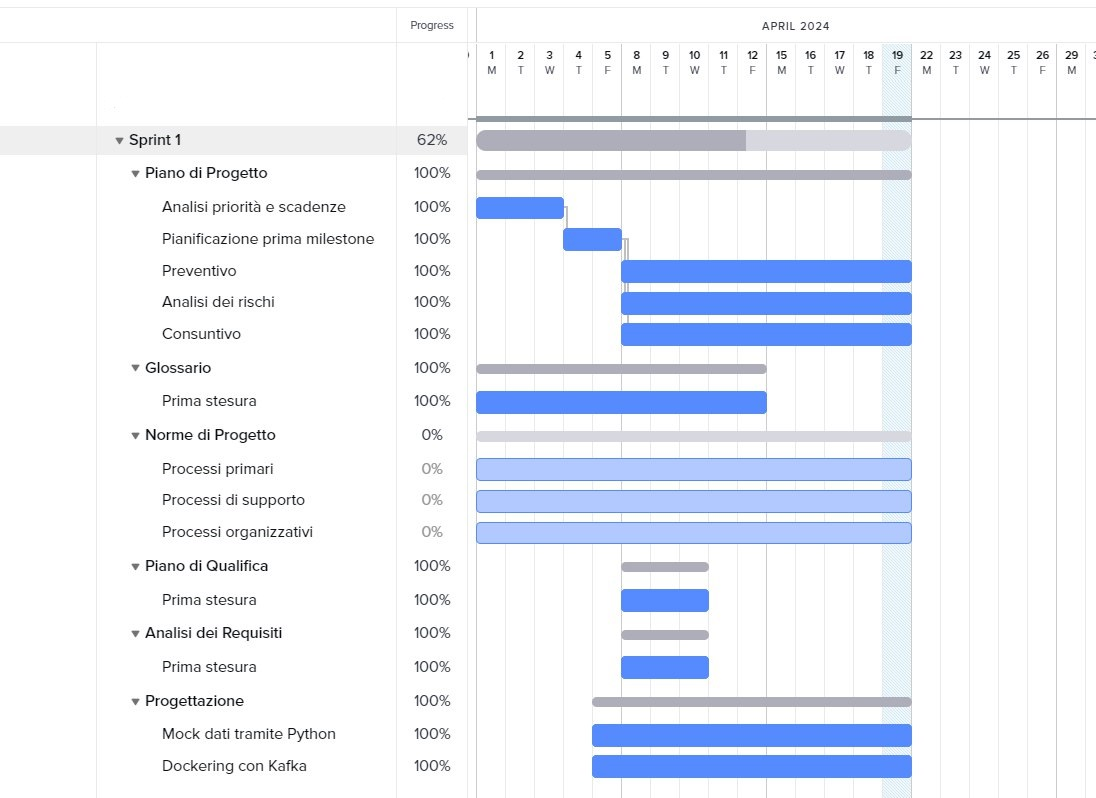
\includegraphics[width=15cm]{./asset/gantt1.jpeg}
    \caption{Diagramma di Gantt rappresentativo del primo periodo.}
    \label{figure:Diagramma di Gantt rappresentativo del primo periodo}
\end{figure}
\clearpage
\newpage
\subsection{Secondo periodo} \label{sec:2_rtb}
\textbf{Inizio:} 2024-04-22\\
\textbf{Fine prevista:} 2024-05-03

\subsubsection{Pianificazione}
In questa fase del processo, assume un'importanza fondamentale condurre un'analisi dettagliata del capitolato al fine di identificare accuratamente i casi d'uso necessari. Inoltre, al fine di evitare ambiguità e decisioni errate, si raccomanda di organizzare uno o più incontri con il proponente per condividere le idee e risolvere i dubbi emersi durante l'analisi, che sarà notevolmente più approfondita rispetto a quella svolta durante la selezione del capitolato. Da questo processo di analisi, si darà inizio alla stesura dell'\textit{Analisi dei Requisiti}, un documento di vitale importanza per il progetto poiché conterrà tutti i casi d'uso individuati, nonché i requisiti obbligatori, desiderabili e opzionali.
È altresì consigliabile redigere il \textit{Piano di Qualifica} in questa fase, il quale sarà fondamentale per definire i metodi volti a garantire la qualità dei processi e dei prodotti nel corso dello sviluppo. \\ Seguono le attività previste per questo secondo periodo:
\begin{itemize}
\setlength{\itemsep}{0em}
    \item Conclusione della sezione di Analisi dei Rischi nel documento \textit{Piano di Progetto};
    \item Aggiunta di nuovi termini al \textit{Glossario};
    \item Avvio della stesura delle \textit{Norme di Progetto};
    \item Arricchimento del documento \textit{Piano di Qualifica};
    \item Proseguimento della scrittura dell'\textit{Analisi dei Requisiti};
    \item Sintesi del funzionamento del generatore dati in un documento apposito;
    \item Realizzazione della persistenza dei dati e visualizzazione delle informazioni tramite \glossterm{dashboard}.
\end{itemize}

\subsubsection{Rischi attesi}
In questo secondo periodo prevediamo che si possano manifestare le seguenti problematiche: 
\begin{itemize}
\setlength{\itemsep}{0em}
\item \textbf{RT-1}: Inesperienza;
\item \textbf{RT-2}: Produzione di codice incomprensibile;
\item \textbf{RC-4}: Confusione nella rotazione dei ruoli;
\item \textbf{RP-1}: Stima errata delle tempistiche di progetto;
\item \textbf{RP-2}: Stima errata dei costi di progetto;
\item \textbf{RP-3}: Stima errata del tempo di completamento di un’attività.
\end{itemize}
Alcuni dei rischi identificati sono attribuibili alla limitata esperienza del gruppo, come evidenziato nei verbali, e alla persistenza di lievi difficoltà nello svolgimento delle attività, tra cui la suddivisione dei compiti assegnati. Inoltre, in concomitanza dell'inizio di questo \glossterm{Sprint} avverrà la prima rotazione dei ruoli ricoperti da ciascun membro, da cui deriva l'aggiunta di \textbf{RC-4} ai rischi previsti. Durante lo \glossterm{Sprint} precedente il gruppo ha dimostrato una notevole coesione ed una buona capacità di gestire efficacemente eventuali divergenze di opinioni, pertanto non si è ritenuto necessario mantenere \textbf{RC-3: Conflitti interni} nella lista dei rischi attesi. Infine, è stato aggiunto \textbf{RT-2} per via dell'inizio dello sviluppo del codice per il \glossterm{Proof of Concept} (PoC).
\clearpage
\subsubsection{Preventivo}
\subsubsubsection{Preventivo orario}
\begin{table}[ht!]
	\centering
	\begin{tabular}{p{4cm} p{1cm} p{1cm} p{1cm} p{1cm} p{1cm} p{1cm} p{3cm}}
        \toprule
        \textbf{Membro} & \multicolumn{6}{c}{\textbf{Ruoli}} & \textbf{Totale (persona)}\\
		& \textbf{AM} & \textbf{RE} & \textbf{PT} & \textbf{AN} & \textbf{PR} & \textbf{VE}\\
		\midrule
        Linda Barbiero          & 3     & -     & 2     & -     & 4     & 3     & 12 \\
        Guglielmo Barison       & 1     & -     & 2,5     & -     & 2   & 1     & 6,5\\
        Pietro Busato           & 1     & -     & 2,5     & -     & 2   & 1     & 6,5 \\
        Davide Donanzan         & 1     & -     & 2     & 2     & 3     & 1   & 9 \\
        Oscar Konieczny         & -     & -     & 2     & -     & 6     & 1     & 9 \\
        Veronica Tecchiati      & 2     & 3     & -     & 2     & 0     & 1     & 8 \\
        \bottomrule
        \textbf{Totale (ruolo)} & 8     & 3     & 11     & 4   & 17     & 8   & 51 \\
	\end{tabular}
	\caption{Distribuzione delle ore del secondo Sprint secondo ruolo e membro.}
	\label{table:Distribuzione delle ore del secondo Sprint secondo ruolo e membro}
\end{table}
\begin{figure}[ht!]
    \centering
    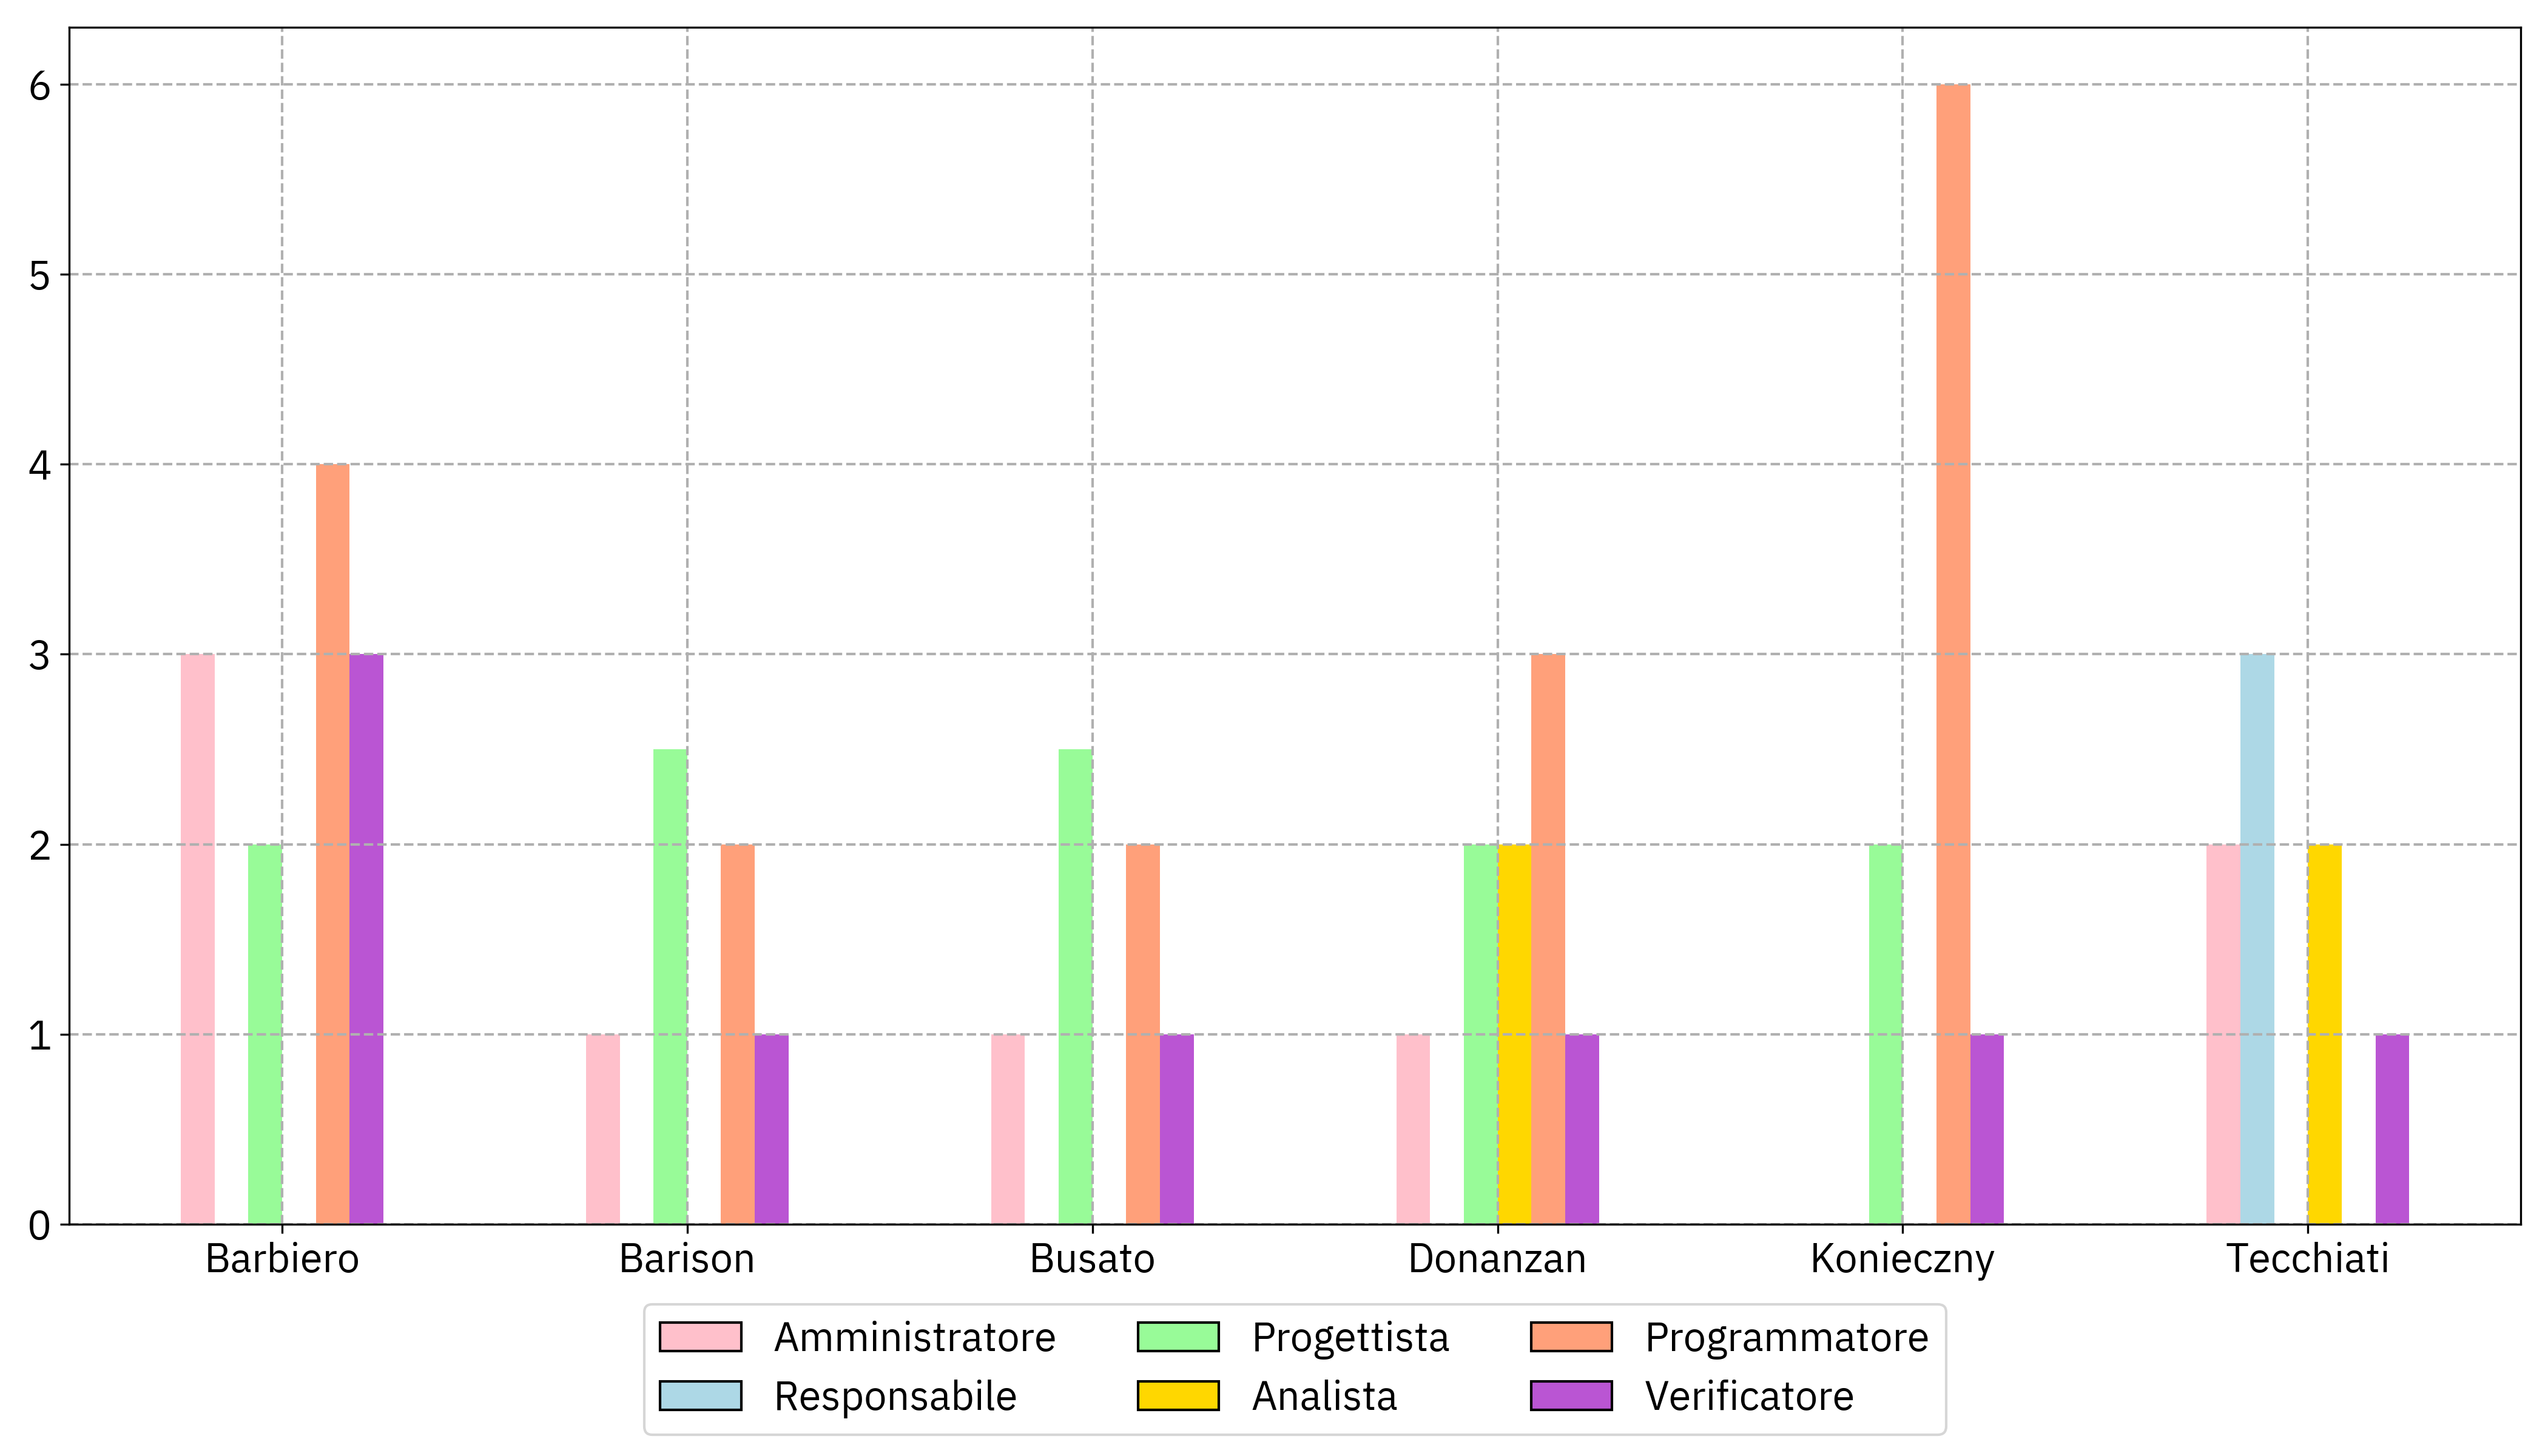
\includegraphics[width=15cm]{./asset/istogramma_periodo_2.png}
    \caption{Visualizzazione dell’impegno temporale di ciascun membro nei rispettivi ruoli assegnati
    nel secondo Sprint.}
    \label{figure:Visualizzazione dell’impegno temporale di ciascun membro nei rispettivi ruoli
    assegnati nel secondo Sprint}
\end{figure}
\subsubsubsection{Preventivo economico}
\begin{table}[ht!]
	\centering
	\begin{tabular}{p{4cm} p{1cm} p{2cm}}
        \toprule
        \textbf{Ruolo} & \textbf{Ore} & \textbf{Costo (€)} \\
        \midrule
        Amministratore & 8 & 240 \\
        Responsabile & 3 & 60 \\
        Progettista & 11 & 275 \\
        Analista & 4 & 100 \\
        Programmatore & 17 & 255 \\
        Verificatore & 8 & 120 \\
        \bottomrule
        \textbf{Totale} & 51 & 1050
    \end{tabular}
    \caption{Preventivo dei costi del secondo Sprint secondo ruolo.}
	\label{table:Preventivo dei costi del secondo Sprint secondo ruolo}
\end{table}
\subsubsection{Consuntivo}
\subsubsubsection{Consuntivo orario}
\begin{table}[ht!]
	\centering
	\begin{tabular}{p{3cm} p{1.4cm} p{1.6cm} p{1.5cm} p{1.5cm} p{1.5cm} p{1.5cm} p{1cm}}
		\toprule
        \textbf{Membro} & \multicolumn{5}{c}{\textbf{Ruoli}} & \multicolumn{2}{r}{\textbf{Totale (pers.)}}\\
		& \textbf{AM} & \textbf{RE} & \textbf{PT} & \textbf{AN} & \textbf{PR} & \textbf{VE}\\
		\midrule
        Linda Barbiero          & 4 \textcolor{red}{(+1)} & - & 1 \textcolor{teal}{(-1)}  & - & 2
        \textcolor{teal}{(-2)} & 3 & 10 \\
        Guglielmo Barison       & - & - & 2,5 & -     & 3 \textcolor{red}{(+1)}  & 1     & 6,5\\
        Pietro Busato           & 1     & -     & 2,5     & -     & 3 \textcolor{red}{(+1)}  & 1     & 7,5 \\
        Davide Donanzan         & - \textcolor{teal}{(-1)}    & -     & 2     & 2     & 2
        \textcolor{teal}{(-1)}     & 1     & 7 \\
        Oscar Konieczny         & -   & -     & 2     & -     & 6     & 1     & 9 \\
        Veronica Tecchiati      & 2   & 3,5 \textcolor{red}{(+0,5)}     & -     & 2     & -     & 1     & 8,5 \\
        \bottomrule
        \textbf{Totale (ruolo)} & 7    & 3,5     & 10     & 4   & 16     & 8   & 48,5 \\
	\end{tabular}
	\caption{Distribuzione delle ore del secondo Sprint secondo ruolo e membro.}
	\label{table:Distribuzione delle ore consuntive del secondo Sprint secondo ruolo e membro}
\end{table}
\begin{table}[ht!]
	\centering
	\begin{tabular}{p{4cm} p{1cm} p{1cm} p{1cm} p{1cm} p{1cm} p{1cm} p{3cm}}
		\toprule
        \textbf{Membro} & \multicolumn{6}{c}{\textbf{Ruoli}} & \textbf{Totale (persona)}\\
		& \textbf{AM} & \textbf{RE} & \textbf{PT} & \textbf{AN} & \textbf{PR} & \textbf{VE}\\
		\midrule
        Linda Barbiero          & 3     & 5     & 19     & 11   & 22     & 19,5   & 79,5 \\
        Guglielmo Barison       & 4     & 9     & 16,5     & 11   & 18,5   & 21     & 80\\
        Pietro Busato           & 5     & 8     & 16,5     & 11   & 17,5   & 21     & 79\\
        Davide Donanzan         & 6     & 8     & 18     & 7    & 21     & 20     & 80\\
        Oscar Konieczny         & 4,5   & 7     & 18     & 11   & 18     & 22     & 80,5\\
        Veronica Tecchiati      & 2,5   & 4,5     & 20     & 4    & 25     & 21     & 77\\
        \bottomrule
        \textbf{Totale (ruolo)} & 25    & 41,5    & 108    & 55   & 122     & 124,5 & 476 \\
	\end{tabular}
	\caption{Ore rimaste dopo il secondo Sprint secondo ruolo e membro.}
	\label{table:Ore rimaste dopo il secondo Sprint secondo ruolo e membro}
\end{table}
\subsubsubsection{Consuntivo economico}
\begin{table}[ht!]
	\centering
	\begin{tabular}{p{4cm} p{2cm} p{2cm}}
        \toprule
        \textbf{Ruolo} & \textbf{Ore} & \textbf{Costo (€)} \\
        \midrule
        Amministratore & 7 \textcolor{teal}{(-1)} & 210 \textcolor{teal}{(-30)}\\
        Responsabile & 3,5 \textcolor{red}{(+0,5)} & 70 \textcolor{red}{(+10)} \\
        Progettista & 10 \textcolor{teal}{(-1)} & 250 \textcolor{teal}{(-25)} \\
        Analista & 4 & 100 \\
        Programmatore & 16 \textcolor{teal}{(-1)} & 240 \textcolor{teal}{(-15)} \\
        Verificatore & 8 & 120 \\
        \bottomrule
        \textbf{Totale} & 48,5 \textcolor{teal}{(-2,5)} & 990 \textcolor{teal}{(-60)}
    \end{tabular}
    \caption{Preventivo a finire dei costi del secondo Sprint secondo ruolo.}
	\label{table:Preventivo a finire dei costi del secondo Sprint secondo ruolo}
\end{table}
\subsubsubsection{Rischi occorsi, impatto e loro mitigazione}
Durante questo periodo sono emerse alcune delle complicazioni previste, in particolar modo quelle riguardanti la pianificazione. Alcune attività hanno subito dei lievi ritardi, il che comporta la necessità di proseguirne lo svolgimento durante lo \glossterm{Sprint} successivo. Inoltre, al termine dello \glossterm{Sprint} è stata rilevata una discrepanza tra i costi preventivati e quelli effettivi, seppure la differenza sia minima. Nonostante ciò, l'impatto complessivo delle suddette problematiche sullo svolgimento del progetto non è da considerarsi allarmante.
\subsubsection{Retrospettiva}
Come anticipato nella sezione precedente, il gruppo ha riscontrato alcune difficoltà legate alla pianificazione. In particolare, l'identificazione e la suddivisione dei nuovi incarichi è avvenuta qualche giorno dopo la data di inizio dello \glossterm{Sprint}, pertanto nei primi giorni il team si è dedicato solamente alla prosecuzione delle attività già avviate nel precedente periodo. In seguito ad un confronto con il Committente, il gruppo ha deciso di introdurre un incontro di \glossterm{Sprint} Planning subito dopo lo svolgimento del SAL con la Proponente, così da delineare immediatamente l'organizzazione del periodo. Nonostante questo iniziale scoglio il gruppo è riuscito comunque a soddisfare le aspettative della Proponente in merito alla scrittura del codice e ad avanzare con la stesura della documentazione. \\
Al termine del secondo periodo è emerso un lieve divario tra i costi previsti e quelli effettivi.
Infatti, il consuntivo riporta una spesa totale di 990\;\texteuro\ anziché i 1\,.050\;\texteuro\ calcolati
nel preventivo. La differenza di 60\;\texteuro\ è dovuta allo svolgimento di un minor quantitativo di
ore da Amministratore, Progettista e Programmatore rispetto alle stime, nonostante il leggero
surplus per il ruolo da Responsabile. Il budget rimanente ammonta dunque a 9\,.352,5\;\texteuro. 
\begin{figure}[h]
    \centering
    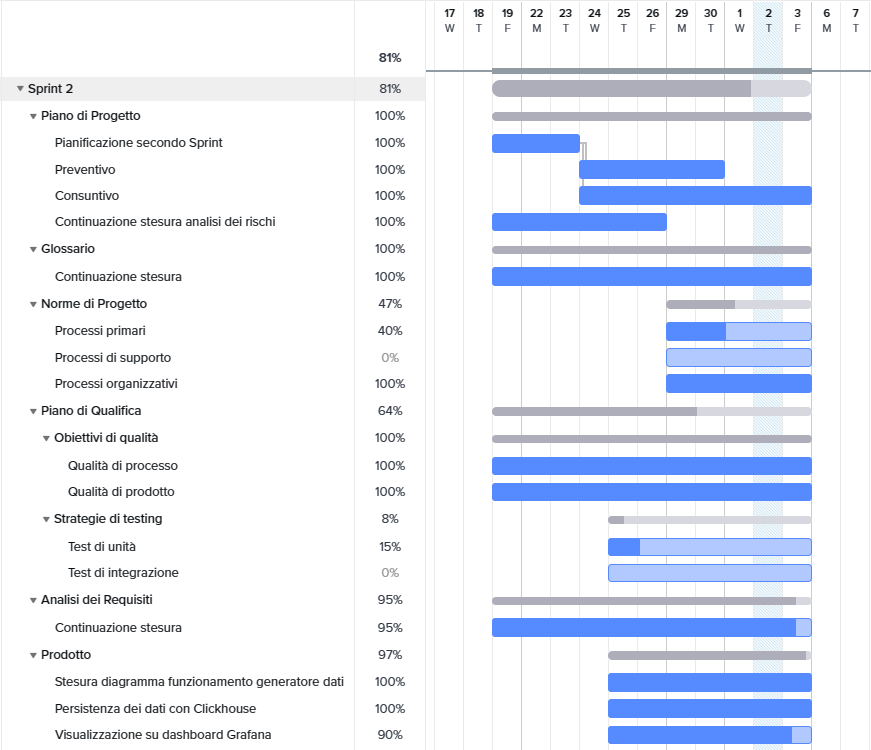
\includegraphics[width=13cm]{./asset/gantt2.png}
    \caption{Diagramma di Gantt rappresentativo del secondo periodo.}
    \label{figure:Diagramma di Gantt rappresentativo del secondo periodo}
\end{figure}
\newpage
\clearpage
\subsection{Terzo periodo} \label{sec:3_rtb}
\textbf{Inizio:} 2024-05-06\\
\textbf{Fine prevista:} 2024-05-17
\subsubsection{Pianificazione}
Con il consolidamento dell'\textit{Analisi dei Requisiti}, diventa fondamentale approfondire gli
strumenti necessari per l'implementazione finale del prodotto. Il \glossterm{Proof of Concept} (PoC) ha
raggiunto un buon grado di avanzamento, anche grazie all'inclusione della componente di
visualizzazione nello \glossterm{Sprint} Backlog, originariamente pianificata per questo periodo.
Prevediamo di completarlo entro il periodo attuale, consentendo così ai programmatori di terminare
il lavoro e successivamente a tutti i membri di dedicarsi al completamento della documentazione, in
vista della prima revisione del progetto. Questo permetterà di realizzare una versione semplificata
del prodotto finale, volta a fornire indicazioni sulla validità della direzione intrapresa e a
dimostrare al committente la correttezza dell'approccio di sviluppo.\\
Considerando il progresso fatto nelle \textit{Norme di Progetto} durante il primo e il secondo
periodo, ora l'attenzione sarà principalmente rivolta a quest'ultime, la cui struttura di base è
stata precedentemente definita. L'obiettivo sarà quello di consolidare ulteriormente il documento,
riflettendo sui dettagli emersi e aggiungendo nuove informazioni.\\
Le attivit\`{a} previste durante questo periodo sono quindi le seguenti:
\begin{itemize}
\setlength{\itemsep}{0em}
    \item Arricchimento del documento \textit{Norme di progetto} precedentemente avviato;
    \item Integrazione della terminologia mancante nel documento \textit{Glossario};
    \item Consolidamento del documento \textit{Analisi dei Requisiti};
    \item Ampliamento del \textit{Piano di Qualifica};
    \item Consolidamento del PoC (\glossterm{Proof of Concept}).
\end{itemize}
\subsubsection{Rischi attesi}
I rischi che ci aspettiamo di correre in questo periodo sono i seguenti: 
\begin{itemize}
\setlength{\itemsep}{0em}
\item \textbf{RT-1:} Inesperienza;
\item \textbf{RP-1:} Stima errata delle tempistiche di progetto;
\item \textbf{RP-2:} Stima errata dei costi di progetto;
\item \textbf{RP-5:} Impegni personali ed accademici;
\end{itemize}
Il consistente carico di lavoro di questo periodo richiederà inevitabilmente più tempo ad ogni membro del gruppo. I rischi identificati sono tecnici ed organizzativi: questi potrebbero causare rallentamenti generali e ritardi.
\clearpage
\subsubsection{Preventivo}
\subsubsubsection{Preventivo orario}
\begin{table}[ht!]
    \centering
    \begin{tabular}{p{4cm} p{1cm} p{1cm} p{1cm} p{1cm} p{1cm} p{1cm} p{3cm}}
        \toprule
        \textbf{Membro} & \multicolumn{6}{c}{\textbf{Ruoli}} & \textbf{Totale (persona)}\\
		& \textbf{AM} & \textbf{RE} & \textbf{PT} & \textbf{AN} & \textbf{PR} & \textbf{VE}\\
		\midrule
        Linda Barbiero       & -   & -   & 2   & -   & 5   & 4   & 11 \\
        Guglielmo Barison    & 2   & 4   & -   & -   & 1   & 2,5 & 9,5 \\
        Pietro Busato        & 4   & -   & -   & 4   & -   & 2   & 10 \\
        Davide Donanzan      & -   & -   & 2   & -   & 5   & 4   & 11 \\
        Oscar Konieczny      & 4   & -   & -   & 4   & -   & 3   & 11 \\
        Veronica Tecchiati   & -   & -   & 2   & -   & 5   & 5   & 12 \\
        \bottomrule
        \textbf{Totali (ruolo)} & 10 & 4 & 6 & 8 & 16 & 20,5 & 64,5 \\
    \end{tabular}
    \caption{Distribuzione delle ore del terzo Sprint secondo ruolo e membro.}
    \label{table:Distribuzione delle ore del terzo Sprint secondo ruolo e membro}
\end{table}
\begin{figure}[ht!]
    \centering
    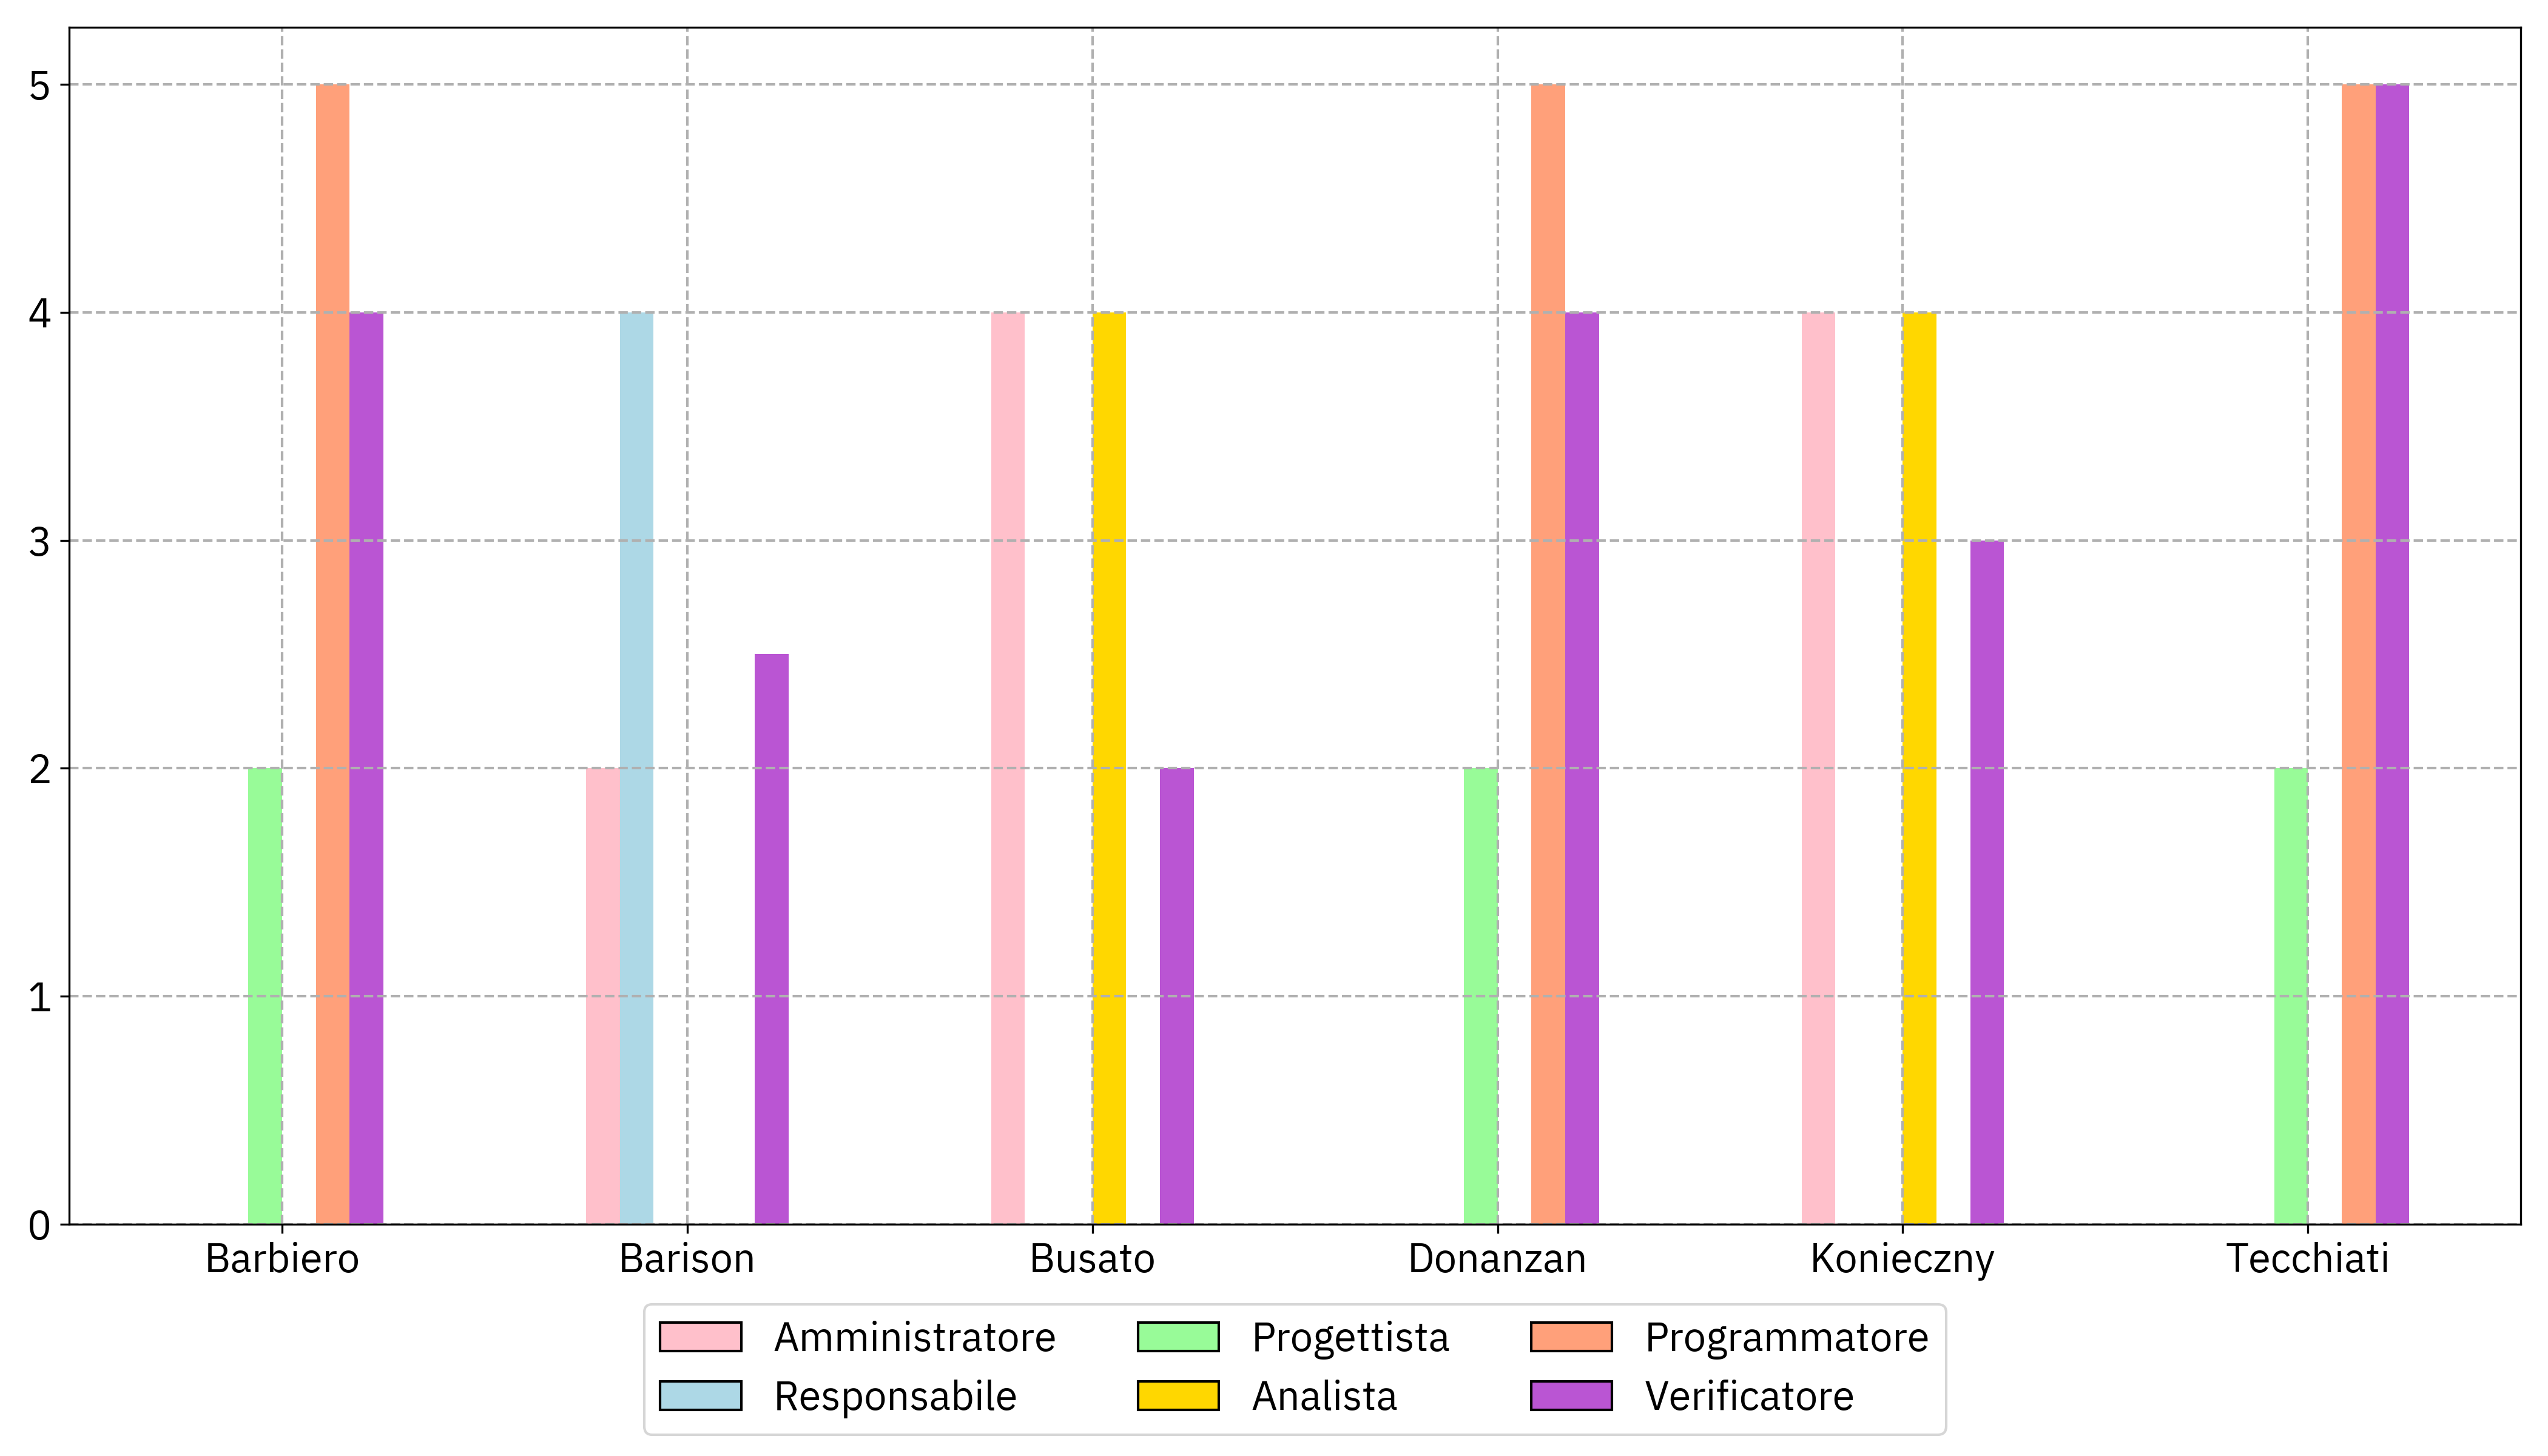
\includegraphics[width=15cm]{./asset/istogramma_periodo_3.png}
    \caption{Visualizzazione dell’impegno temporale di ciascun membro nei rispettivi ruoli assegnati
    nel terzo Sprint.}
    \label{figure:Visualizzazione dell’impegno temporale di ciascun membro nei rispettivi ruoli
    assegnati nel terzo Sprint}
\end{figure}
\subsubsubsection{Preventivo economico}
\begin{table}[ht!]
	\centering
	\begin{tabular}{p{4cm} p{1cm} p{2cm}}
        \toprule
        \textbf{Ruolo} & \textbf{Ore} & \textbf{Costo (€)} \\
        \midrule
        Amministratore & 10 & 300 \\
        Responsabile & 4 & 80 \\
        Progettista & 6 & 150 \\
        Analista & 8 & 200 \\
        Programmatore & 16 & 240 \\
        Verificatore & 20.5 & 307,5 \\
        \bottomrule
        \textbf{Totale} & 64,5 & 1277,5
    \end{tabular}
    \caption{Preventivo dei costi del terzo Sprint secondo ruolo.}
	\label{table:Preventivo dei costi del terzo Sprint secondo ruolo}
\end{table}
\subsubsection{Consuntivo}
\subsubsubsection{Consuntivo orario}
\begin{table}[ht!]
	\centering
	\begin{tabular}{p{3cm} p{1.4cm} p{1.6cm} p{1.7cm} p{1.4cm} p{1.4cm} p{1.5cm} p{2cm}}
		\toprule
        \textbf{Membro} & \multicolumn{5}{c}{\textbf{Ruolo}} & \multicolumn{2}{r}{\textbf{Totale (persona)}}\\
		& \textbf{AM} & \textbf{RE} & \textbf{PT} & \textbf{AN} & \textbf{PR} & \textbf{VE}\\
		\midrule
        Linda Barbiero     & - & - & 2 & -   & 5 & 4 & 11 \\
        Gugliemo Barison   & 2 & 4 & - & -   & 1 & 2,5 & 9,5 \\
        Pietro Busato      & 3 \textcolor{teal}{(-1)} & - & - & 3.5
        \textcolor{red}{(-1.5)} & - & 1 \textcolor{teal}{(-1)} & 7,5 \\
        Davide Donanzan    & - & - & 2 & -   & 5 & 4 & 11 \\
        Oscar Konieczny    & 4 & - & - & 4   & - & 3 & 11 \\
        Veronica Tecchiati & 1 \textcolor{red}{(+1)} & -  & 2 & -   & 3 \textcolor{teal}{(-2)} & 4
        \textcolor{teal}{(-1)}  & 10 \\
        \midrule
        \textbf{Totale (ruolo)} & 10 & 4 & 6 & 7,5 & 14 & 18,5 & 60 \\
		\bottomrule
	\end{tabular}
	\caption{Distribuzione delle ore del terzo Sprint secondo ruolo e membro.}
	\label{table:Distribuzione delle ore del terzo Sprint secondo ruolo e membr}
\end{table}
\begin{table}[ht!]
	\centering
	\begin{tabular}{p{3cm} p{1.4cm} p{1.6cm} p{1.5cm} p{1.5cm} p{1.5cm} p{1.5cm} p{2cm}}
		\toprule
        \textbf{Membro} & \multicolumn{5}{c}{\textbf{Ruolo}} & \multicolumn{2}{r}{\textbf{Totale (persona)}}\\
		& \textbf{AM} & \textbf{RE} & \textbf{PT} & \textbf{AN} & \textbf{PR} & \textbf{VE}\\
		\midrule
        Linda Barbiero     & 3 & 5 & 17 & 11   & 17 & 15,5 & 68,5 \\
        Gugliemo Barison   & 2 & 5 & 16,5 & 11   & 17,5 & 18,5 & 70,5 \\
        Pietro Busato      & 2 & 8 & 16,5 & 7,5 & 17,5 & 20 & 71,5 \\
        Davide Donanzan    & 6 & 8 & 16 & 7   & 16 & 16 & 69 \\
        Oscar Konieczny    & 0,5 & 7 & 18 & 7   & 18 & 19 & 69,5 \\
        Veronica Tecchiati & 1,5 & 4,5 & 18 & 4   & 22 & 17 & 67 \\
        \midrule
        \textbf{Totale (ruolo)} & 15 & 37,5 & 102 & 47,5 & 108 & 106 & 416 \\
		\bottomrule
	\end{tabular}
	\caption{Ore rimaste dopo il terzo Sprint secondo ruolo e membro.}
	\label{table:Ore rimaste dopo il terzo Sprint secondo ruolo e membro.}
\end{table}
\subsubsubsection{Consuntivo economico}
\begin{table}[ht!]
    \centering
    \begin{tabular}{p{4cm} p{1.8cm} p{2.2cm}}
        \toprule
        \textbf{Ruolo} & \textbf{Ore} & \textbf{Costo (€)} \\
        \midrule
        Amministratore & 10 & 300 \\
        Responsabile & 4  & 80 \\
        Progettista & 6  & 150 \\
        Analista & 7,5 \textcolor{teal}(-0,5) & 187,5 \textcolor{teal}{(-12,5)}\\
        Programmatore & 14 \textcolor{red}{(-1)} & 210 \textcolor{teal}{(-15)}\\
        Verificatore & 18,5 \textcolor{red}{(+1,5)} & 277,5 \textcolor{red}{(+30)} \\
        \bottomrule
        \textbf{Totale} & 60 & 1205
    \end{tabular}
    \caption{Preventivo a finire dei costi del terzo Sprint secondo ruolo.}
    \label{table:Preventivo a finire dei costi del terzo Sprint secondo ruolo}
\end{table}

\subsubsubsection{Rischi occorsi, impatto e loro mitigazione}
\\Nel corso di questo periodo il gruppo ha scelto di svolgere numerose attivit\`{a} in un tempo limitato.
In seguito ad un controllo generale della documentazione, sono emerse diverse imprecisioni in
particolari sezioni, sottolineando come alcune attivit\`{a} non fossero state svolte in maniera
ottimale. Gli analisti si sono occupati di sistemare queste parti. I rischi preventivati hanno avuto un impatto medio sul gruppo, causando principalmente stress, tuttavia, alla fine, sono stati mitigati nel miglior modo possibile.
\subsubsection{Retrospettiva}
Il terzo periodo si è rivelato, come da aspettative, il pi\`{u} intenso dei tre. Tutto sommato, il
carico di lavoro poteva essere distribuito diversamente, magari su pi\`{u} periodi di lavoro.
All'interno del team, è stato notevolmente valutato l'impegno di alcuni membri nel dedicare
ulteriori ore per prevenire un rallentamento eccessivo nell'avanzamento globale del progetto.
Tuttavia, sarebbe auspicabile evitare tali circostanze in futuro, sebbene abbiano messo in luce la
determinazione della maggioranza del gruppo a procedere con decisione.\\
Al termine del secondo periodo è emerso un lieve divario tra i costi previsti e quelli effettivi.
Infatti, il consuntivo riporta una spesa totale di 1\,.205\;\texteuro\ anzichè i 1\,.277,5\;\texteuro\ calcolati
nel preventivo. La differenza di 72,5\;\texteuro\ è dovuta all'indisposizione fisica di uno dei membri del gruppo, impossibilitato quindi a portare a termine tutte le ore assegnategli. Il budget rimanente ammonta dunque a 8\,.147,5\;\texteuro.
\begin{figure}[h!]
    \centering
    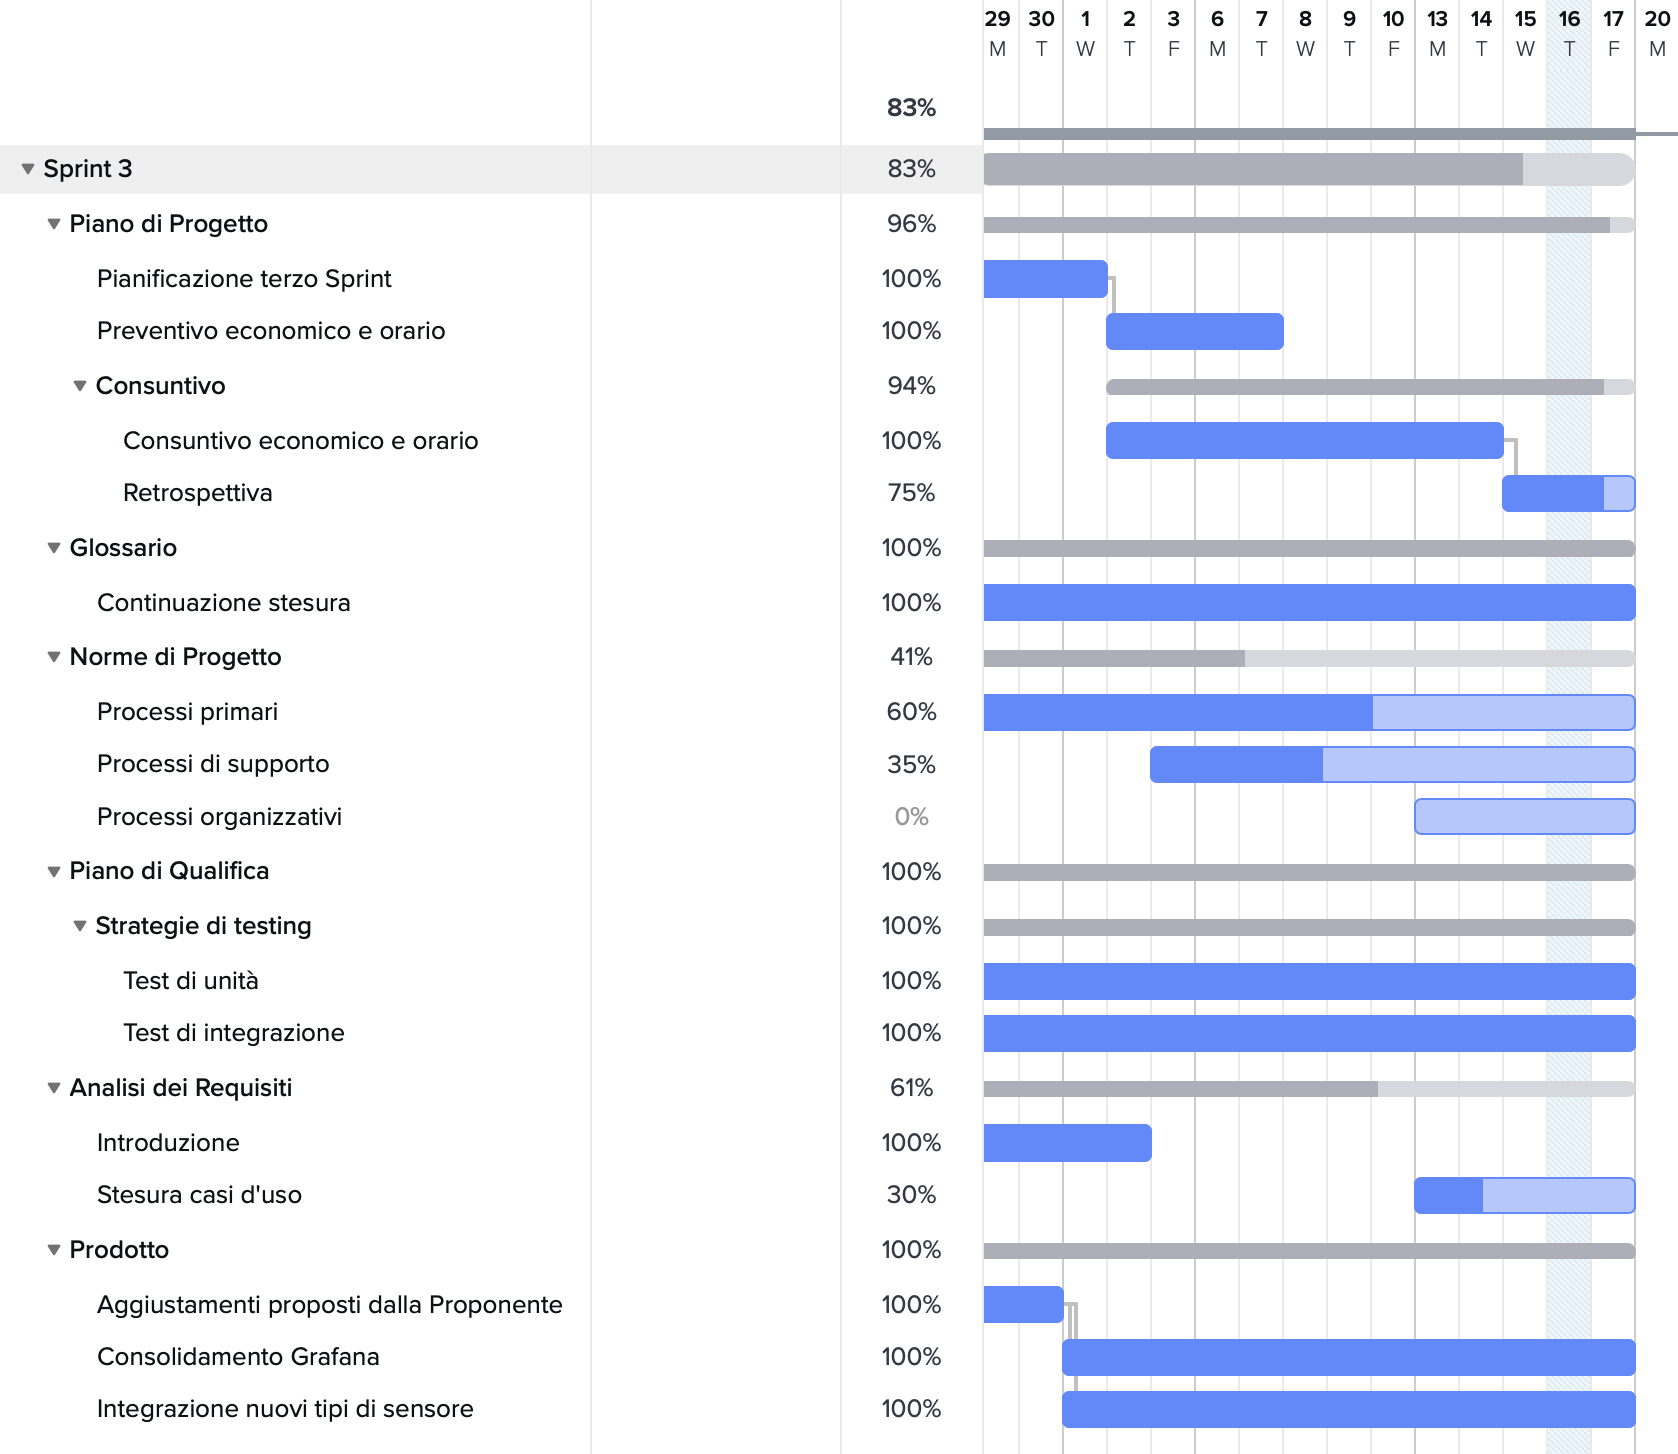
\includegraphics[width=13cm]{./asset/gantt3.png}
    \caption{Diagramma di Gantt rappresentativo del terzo periodo.}
\end{figure}
\clearpage
\subsection{Quarto periodo} \label{sec:4_rtb}
\textbf{Inizio:} 2024-05-20\\
\textbf{Fine prevista:} 2024-05-31
\subsubsection{Pianificazione}
Essendo questo l'ultimo Sprint di due settimane complete prima della fine della prima parte del progetto,
con conseguente presentazione del \textit{PoC}, assume primaria importanza l'ultimazione della progettazione
e implementazione di quest'ultimo, nonché una rifinitura dello stesso. Parallelamente, diventano imprescindibili
il completamento, il perfezionamento e la verifica finale di tutti documenti in vista della revisione pianificata
per l'inizio del mese di giguno. \\
Il mancato chiarimento con l'azienda proponente dell'implementazione e funzionamento di una parte del progetto,
con conseguente riscrittura e implementazione di una non indifferente porzione di codice, pone tuttavia un pericoloso
contrattempo e aggiunge una difficoltà da risolvere che va ad accatastarsi su una mole di lavoro già massicia. \\
L'avvicinamento inoltre del periodo di esami di inizio estate aggiunge infine ulteriore pressione e precarietà
alla situazione, che il team si ritiene comunque pronto ad affrontare con determinazione e grinta.\\
Le attività previste durante questo periodo sono quindi le seguenti:
\begin{itemize}
\setlength{\itemsep}{0}
    \item ristrutturazione e reimplementazione di parte del progetto;
    \item rifinitura e pulitura del prodotto da presentare, ovvero il \textit{PoC};
    \item completamento della documentazione;
    \item rifinitura e pulitura della documentazione.
\end{itemize}
\subsubsection{Rischi attesi}
I rischi che ci aspettiamo di correre in questo periodo sono i seguenti: 
\begin{itemize}
\setlength{\itemsep}{0}
    \item \textbf{RT-1} Inesperienza;  
    \item \textbf{RC-2} Scarsa comunicazione con la proponente;
    \item \textbf{RP-2} Stima errata dei costi di progetto;
    \item \textbf{RP-3} Stima errata del tempo di completamento di un'attività;
    \item \textbf{RP-5} Impegni personali ed accademici.
\end{itemize}
\subsubsection{Preventivo}
\subsubsubsection{Preventivo orario}
\begin{table}[ht!]
	\centering
	\begin{tabular}{p{4cm} p{1cm} p{1cm} p{1cm} p{1cm} p{1cm} p{1cm} p{3cm}}
		\toprule
        \textbf{Membro} & \multicolumn{6}{c}{\textbf{Ruoli}} & \textbf{Totale (persona)}\\
		& \textbf{AM} & \textbf{RE} & \textbf{PT} & \textbf{AN} & \textbf{PR} & \textbf{VE}\\
		\midrule
        Linda Barbiero          & 2     & -     & 4     & 7     & 4     & 3     & 22 \\
        Guglielmo Barison       & 1     & -     & 4     & 3     & 4     & 3     & 15\\
        Pietro Busato           & 4     & 4     & 4     & 0     & 4     & 3     & 19 \\
        Davide Donanzan         & 1     & -     & 4     & 3     & 6     & 3     & 17 \\
        Oscar Konieczny         & 4     & -     & 4     & 0     & 3     & 3     & 14 \\
        Veronica Tecchiati      & 2     & -     & 4     & 5     & 1,5   & 3     & 15,5 \\
        \bottomrule
        \textbf{Totale (ruolo)} & 16    & 4     & 24    & 18    & 22,5  & 18   & 100,5 \\
	\end{tabular}
	\caption{Distribuzione delle ore del quarto Sprint secondo ruolo e membro.}
	\label{table:Distribuzione delle ore del quarto Sprint secondo ruolo e membro}
\end{table}
%\begin{figure}[ht!]
%    \centering
%    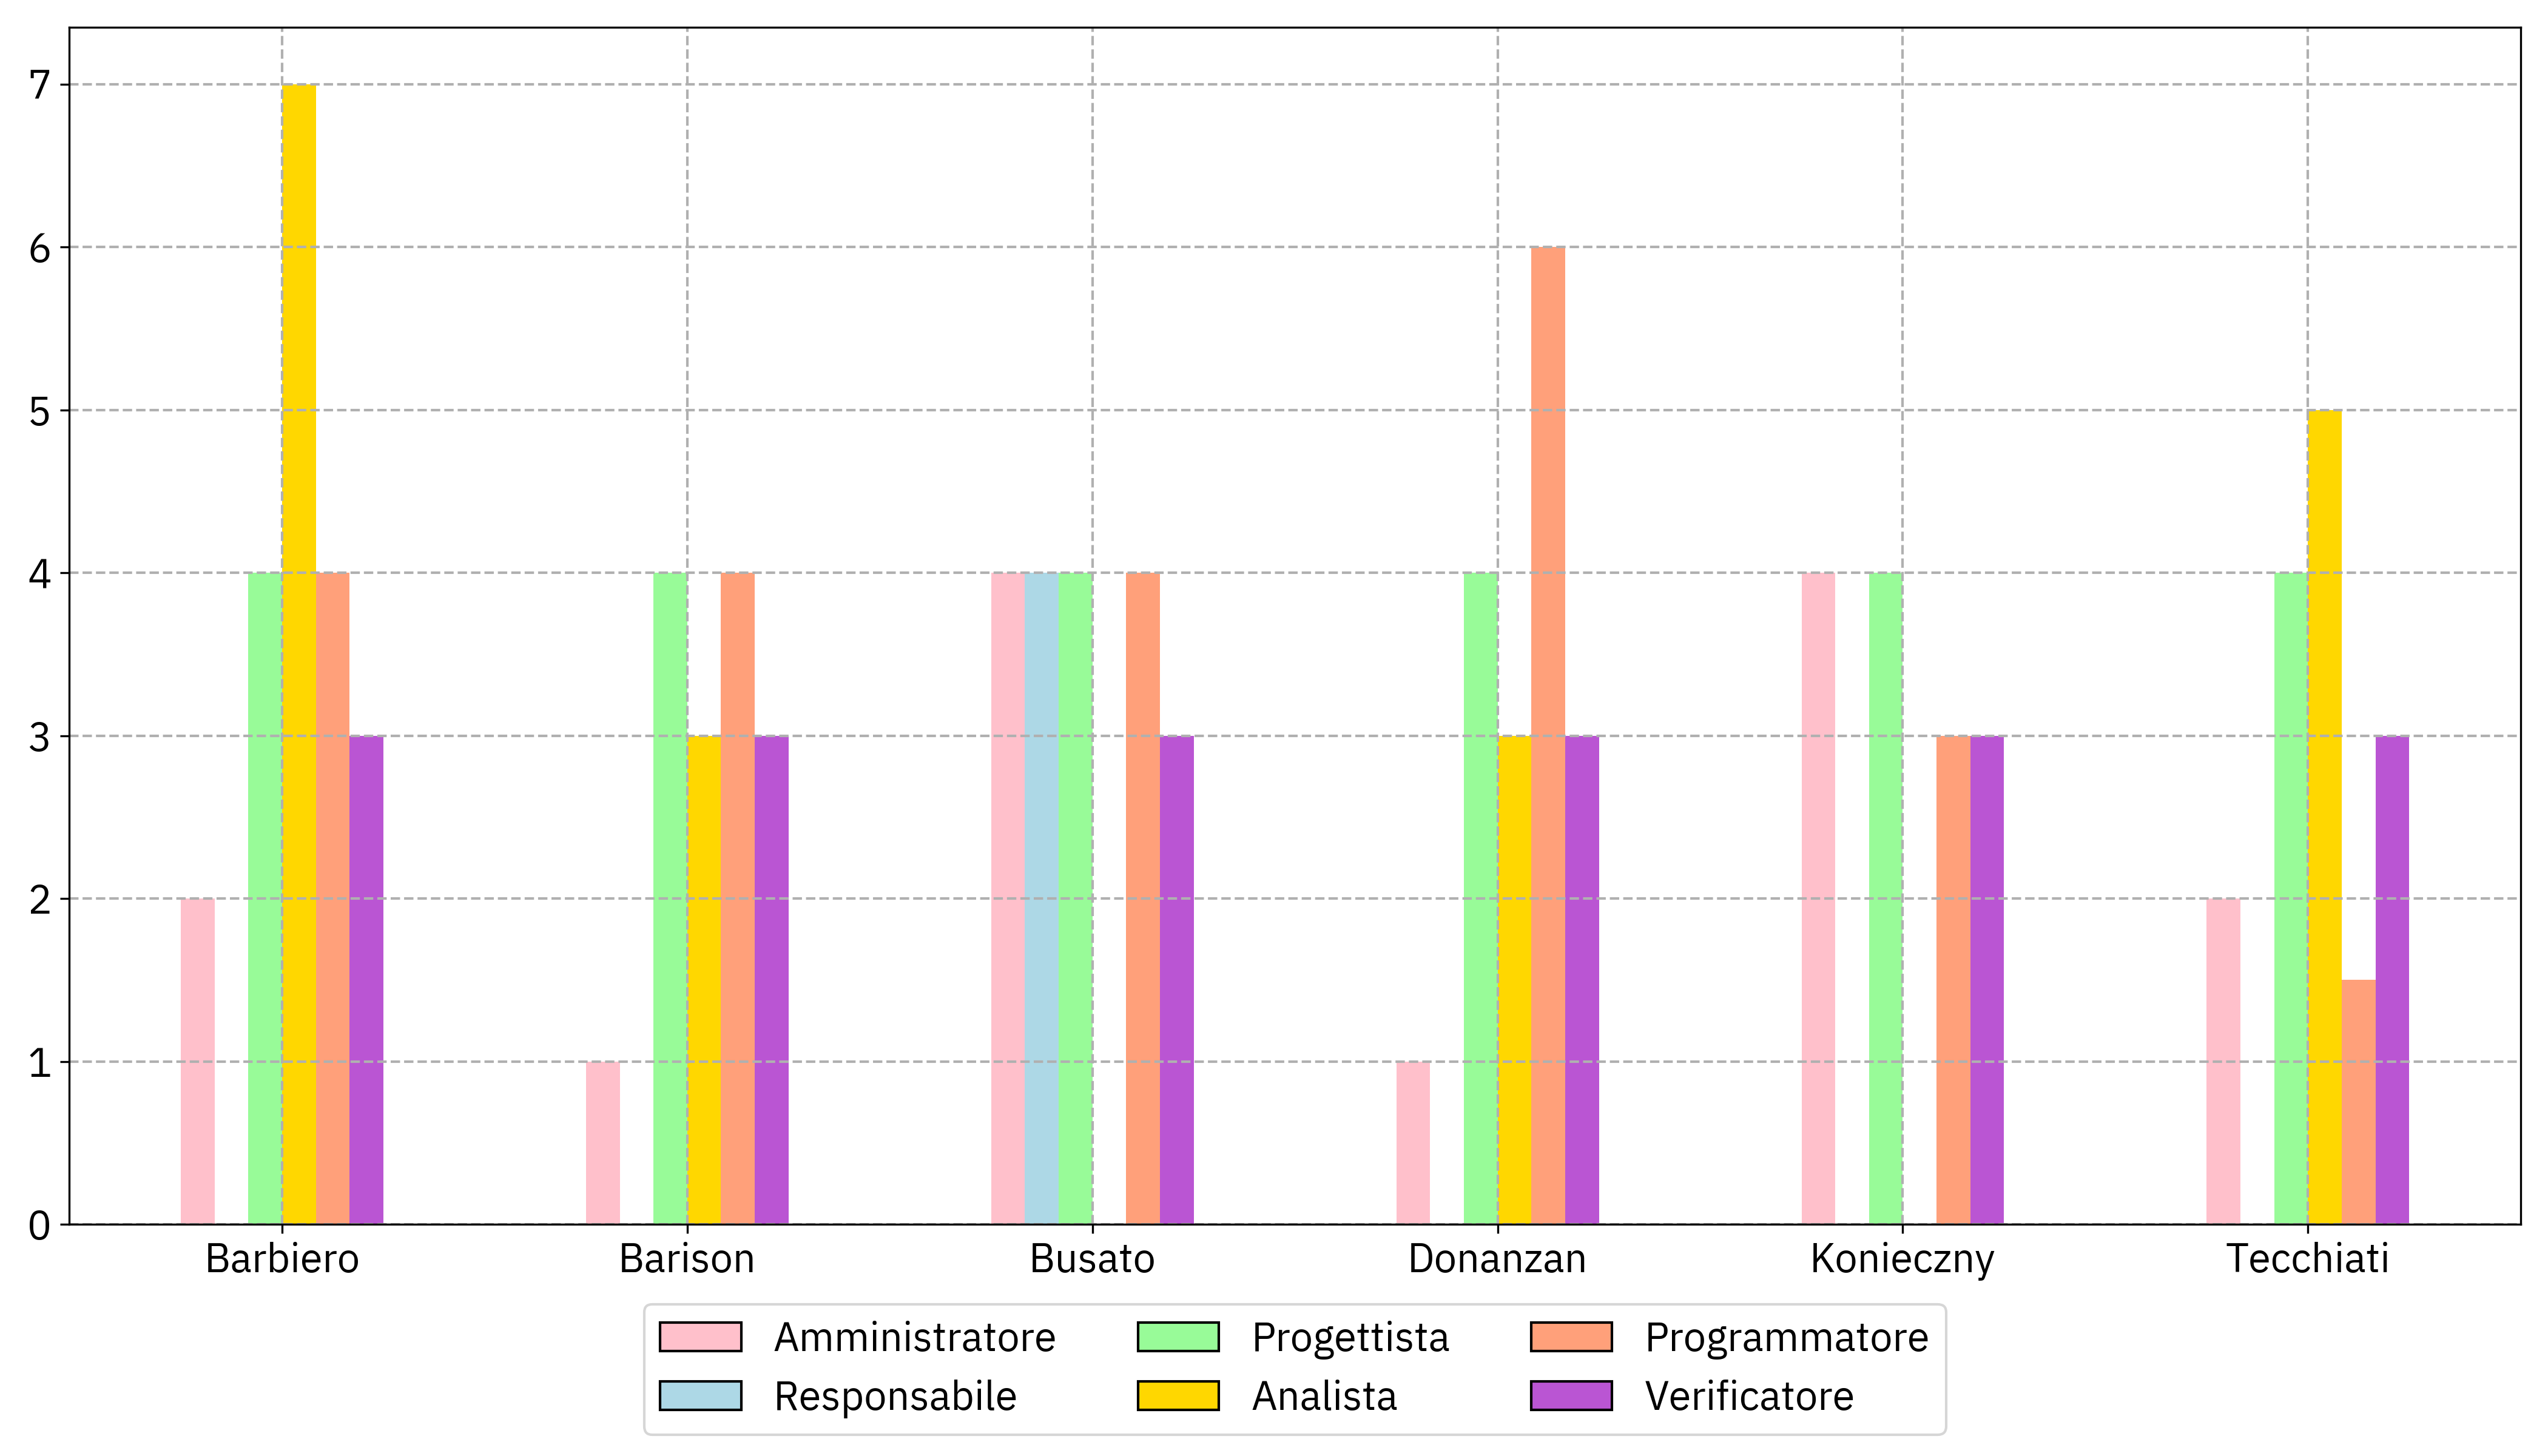
\includegraphics[width=15cm]{./asset/istogramma_periodo_4.png}
%    \caption{Visualizzazione dell’impegno temporale di ciascun membro nei rispettivi ruoli assegnati
%    nel terzo Sprint.}
%    \label{figure:Visualizzazione dell’impegno temporale di ciascun membro nei rispettivi ruoli
%    assegnati nel terzo Sprint}
%\end{figure}
\subsubsubsection{Preventivo economico}
\begin{table}[ht!]
	\centering
	\begin{tabular}{p{4cm} p{1cm} p{2cm}}
        \toprule
        \textbf{Ruolo} & \textbf{Ore} & \textbf{Costo (€)} \\
        \midrule
        Amministratore & 14 & 420 \\
        Responsabile & 4 & 80 \\
        Progettista & 24 & 600 \\
        Analista & 18 & 450 \\
        Programmatore & 22,5 & 337,5 \\
        Verificatore & 18 & 270 \\
        \bottomrule
        \textbf{Totale} & 100,5 & 2157,5
    \end{tabular}
    \caption{Preventivo dei costi del quarto Sprint secondo ruolo.}
	\label{table:Preventivo dei costi del quarto Sprint secondo ruolo}
\end{table}
\subsubsection{Consuntivo}
\subsubsubsection{Consuntivo orario}
\begin{table}[ht!]
	\centering
	\begin{tabular}{p{3cm} p{1.4cm} p{1.6cm} p{1.7cm} p{1.4cm} p{1.4cm} p{1.5cm} p{2cm}}
		\toprule
        \textbf{Membro} & \multicolumn{5}{c}{\textbf{Ruolo}} & \multicolumn{2}{r}{\textbf{Totale (persona)}}\\
		& \textbf{AM} & \textbf{RE} & \textbf{PT} & \textbf{AN} & \textbf{PR} & \textbf{VE}\\
		\midrule
        Linda Barbiero     & 1\textcolor{teal}{(-1)} & - & 3\textcolor{teal}{(-1)} & 5\textcolor{teal}{(-2)} & 5\textcolor{red}{(+1)} & 3 & 17\textcolor{teal}{(-3)} \\
        Gugliemo Barison   & 1 & - & 2\textcolor{teal}{(-2)} & 4\textcolor{red}{(+1)} & 6\textcolor{red}{(+2)} & 3,5\textcolor{red}{(+0,5)} & 16.5\textcolor{red}{(+1,5)} \\
        Pietro Busato      & 3\textcolor{teal}{(-1)} & 4 & 2\textcolor{teal}{(-2)} & 4\textcolor{red}{(+4)} & 5\textcolor{red}{(+1)} & 3 & 21\textcolor{red}{(+2)} \\
        Davide Donanzan    & 1 & - & 4 & 5\textcolor{red}{(+2)} & 7\textcolor{red}{(+1)} & 3 & 20\textcolor{red}{(+3)} \\
        Oscar Konieczny    & 3\textcolor{teal}{(-1)} & - & 3\textcolor{teal}{(-1)} & 3\textcolor{red}{(+3)} & 3.5\textcolor{red}{(+0,5)} & 4\textcolor{red}{(+1)} & 16.5\textcolor{red}{(+2,5)}\\
        Veronica Tecchiati & -\textcolor{teal}{(-2)} & - & 1\textcolor{teal}{(-3)} & 4\textcolor{teal}{(-1)} & 4\textcolor{red}{(+2,5)} & 4\textcolor{red}{(+1)} & 13\textcolor{teal}{(-2,5)} \\
        \midrule
        \textbf{Totale (ruolo)} & 9 & 4 & 15 & 25 & 30.5 & 20,5 & 104 \\
		\bottomrule
	\end{tabular}
	\caption{Distribuzione delle ore del quarto Sprint secondo ruolo e membro.}
	\label{table:Distribuzione delle ore del terzo Sprint secondo ruolo e membr}
\end{table}
\begin{table}[ht!]
	\centering
	\begin{tabular}{p{3cm} p{1.4cm} p{1.6cm} p{1.5cm} p{1.5cm} p{1.5cm} p{1.5cm} p{2cm}}
		\toprule
        \textbf{Membro} & \multicolumn{5}{c}{\textbf{Ruolo}} & \multicolumn{2}{r}{\textbf{Totale (persona)}}\\
		& \textbf{AM} & \textbf{RE} & \textbf{PT} & \textbf{AN} & \textbf{PR} & \textbf{VE}\\
		\midrule
        Linda Barbiero     & 2 & 5 & 14 & 6 & 12 & 12,5 & 68,5 \\
        Gugliemo Barison   & 1 & 5 & 14,5 & 7 & 11,5 & 15 & 54 \\
        Pietro Busato      & -1& 4 & 14,5 & 3,5 & 12,5 & 17 & 50,5 \\
        Davide Donanzan    & 5 & 8 & 12 & 2 & 9 & 13 & 49 \\
        Oscar Konieczny    & -2,5 & 7 & 15 & 4 & 14,5 & 15 & 53 \\
        Veronica Tecchiati & 1,5 & 4,5 & 17 & 0 & 18 & 13 & 54 \\
        \midrule
        \textbf{Totale (ruolo)} & 6 & 33,5 & 87 & 22,5 & 77 & 85,5 & 312 \\
		\bottomrule
	\end{tabular}
	\caption{Ore rimaste dopo il quarto Sprint secondo ruolo e membro.}
	\label{table:Ore rimaste dopo il terzo Sprint secondo ruolo e membro.}
\end{table}
\subsubsubsection{Consuntivo economico}
in{table}[ht!]
    \centering
    \begin{tabular}{p{4cm} p{1.8cm} p{2.2cm}}
        \toprule
        \textbf{Ruolo} & \textbf{Ore} & \textbf{Costo (€)} \\
        \midrule
        Amministratore & 9\textcolor{teal}(-5) & 270\textcolor{teal}(-150) \\
        Responsabile & 4  & 80 \\
        Progettista & 15\textcolor{teal}(-9)  & 375\textcolor{teal}(-225) \\
        Analista & 25\textcolor{red}(+7) & 625\textcolor{red}(+175) \\
        Programmatore & 30,5\textcolor{red}(+8) & 457,5\textcolor{red}(+120) \\
        Verificatore & 20,5\textcolor{red}(+2,5) & 307,5\textcolor{red}(+37,5) \\
        \bottomrule
        \textbf{Totale} & 104 & 2115
    \end{tabular}
    \caption{Preventivo a finire dei costi del quarto Sprint secondo ruolo.}
    \label{table:Preventivo a finire dei costi del terzo Sprint secondo ruolo}
\end{table}
\subsubsubsection{Rischi occorsi, impatto e loro mitigazione}
Questo Sprint ha visto susseguirsi numerose problematiche, principalmente riguardanti
il tempo a disposizione rispetto al carico di lavoro assegnato. Ciononostante, il team ha svolto compiti e risolto problemi con celerità
e determinazione, riuscendo a garantire il completamento degli obiettivi fissati entro il tempo
limite. Questo tuttavia ha portato il gruppo a dover redistribuire alcuni carichi di lavoro e
riassegnare parzialmente i ruoli in itinere: ne consegue che il consuntivo differisce discretamente 
dal preventivo e, sebbene da un punto di vista economico si sia riusciti a risparmiare una piccola somma
di denaro -42,5\texteuro, il monte ore finale presenta uno scenario abbastanza diverso da quello previsto.
Un altro problema verificatosi durante lo Sprint, conseguente al ritmo accelerato di lavoro che ci si è stati trovati ad adottare, 
risiede nell'aver giocoforza rivolto minore attenzione alla cura dei dettagli di alcune parti di documentazione, che il team 
si è già riservato di ottemperare nel prossimo Sprint, della durata prevista di una singola settimana, in preparazione all'RTB.
\subsubsection{Retrospettiva}
Come già precedentemente accennato, durante questo Sprint il team ha dimostrato conretamente di essere in grado di gestire in maniera adeguata
situazioni improvvise, perigliose e stringenti, con l'unica pecca di aver dovuto, in alcuni momenti, gestire i ruoli e le ore assegnate
a ciascun membro in maniera riorganizzata, sia per problemi di compatibilità con impegni personali, sia per semplificare la risoluzione 
dei vari compiti sulla base delle conoscenze pregresse e del lavoro svolto fino a quel momento da ciascuno. Al netto di essere riusciti a
mantenere pressocchè inalterato il costo finale dello Sprint e di non aver subito rallentamenti rilevanti per quanto riguarda l'avanzamento
del progetto, il gruppo dovrà tuttavia impegnarsi più a fondo per quanto riguarda la comunicazione con la Proponente e il chiarimento
di eventuali dubbi sorti durante gli incontri, siano essi SAL o diari di bordo: il team dovrà fare più affidamento sui canali di comunicazione
per discutere con l'azienda di probabili misinterpretazioni o mancati chiarimenti, e non esitare a chiedere consiglio ai Prof. Vardanega e Cardin,
per risolvere preventivamente o evitare completamente, in futuro, situazioni simili. 
\begin{figure}[h!]
    \centering
    \includegraphics[width=13cm]{./asset/gantt4.png}
    \caption{Diagramma di Gantt rappresentativo del quarto periodo.}
\end{figure}
\clearpage
